\documentclass[12pt,addpoints,answers]{repaso}
\grado{1}
\nivel{Secundaria}
\cicloescolar{2024-2025}
\materia{Matemáticas}
\unidad{3}
\title{Practica la Unidad}
\aprendizajes{\footnotesize%
      \item Verifica algebraicamente la equivalencia de expresiones de primer grado, formuladas a partir de sucesiones.
      \item Resuelve problemas mediante la formulación y solución algebraica de ecuaciones lineales.
      \item Usa e interpreta las medidas de tendencia central (moda, media aritmética y mediana).
      \item Calcula el área y volumen de piramides, prismas y cilindros rectos.
      \item Calcula el perímetro y el área de polígonos regulares y del círculo a partir de diferentes datos.
}
\author{Melchor Pinto, J.C.}
\begin{document}
\INFO
\section*{Sucesiones}
\subsection*{Completa la sucesión aritmética}

\ejemplosboxed[{Escribe los términos faltantes de las siguientes sucesiones aritméticas:

                  \begin{multicols}{3}
                        \begin{parts}
                              \part 28, 39, 50, \fillin[61][0.5cm], \fillin[72][0.5cm], \fillin[84][0.5cm], \dots
                              \part 56, 50, 44, \fillin[38][0.5cm], \fillin[32][0.5cm], \fillin[26][0.5cm], \dots
                              \part 33, 41, 49, \fillin[57][0.5cm], \fillin[65][0.5cm], \fillin[73][0.5cm], \dots
                        \end{parts}
                  \end{multicols}%
            }]

\begin{questions}
      \questionboxed[6]{Escribe los términos faltantes de las siguientes sucesiones aritméticas:

            \begin{multicols}{3}
                  \begin{parts}
                        \part 21, 25, 29, \fillin[33][0.5cm], \fillin[37][0.5cm], \fillin[41][0.5cm], \dots
                        % \part  4, 10, 16, \fillin[22][0.5cm], \fillin[28][0.5cm], \fillin[34][0.5cm], \dots
                        \part 34, 31, 28, \fillin[25][0.5cm], \fillin[22][0.5cm], \fillin[19][0.5cm], \dots
                        \part 92, 86, 80, \fillin[74][0.5cm], \fillin[68][0.5cm], \fillin[62][0.5cm], \dots
                        % \part 51, 46, 41, \fillin[36][0.5cm], \fillin[31][0.5cm], \fillin[26][0.5cm], \dots
                        % \part 250,225,200, \fillin[175][0.5cm], \fillin[150][0.5cm], \fillin[125][0.5cm], \dots
                  \end{parts}
            \end{multicols}
      }

      % \subsection*{Completa la sucesión aritmética 2}

      \ejemplosboxed[{Escribe los primeros 4 términos de las siguientes sucesiones aritméticas:

                        \begin{multicols}{3}
                              \begin{parts}
                                    \part $a_n=7n+4$ \\ \fillin[11][0.5cm], \fillin[18][0.5cm], \fillin[25][0.5cm], \fillin[32][0.5cm], \dots
                                    \part $a_n=-5n+15 $ \\  \fillin[10][0.5cm], \fillin[5][0.5cm], \fillin[0][0.5cm], \fillin[-5][0.5cm], \dots
                                    \part $a_n=-n-5$  \\  \fillin[-6][0.5cm], \fillin[-7][0.5cm], \fillin[-8][0.5cm], \fillin[-9][0.5cm], \dots
                              \end{parts}
                        \end{multicols}
                  }]

      \questionboxed[6]{Escribe los primeros 4 términos de las siguientes sucesiones aritméticas:

            \begin{multicols}{3}
                  \begin{parts}
                        \part
                        $a_n=-7n+5$ \\ \fillin[-2][0.5cm], \fillin[-9][0.5cm], \fillin[-16][0.5cm], \fillin[-23][0.5cm], \dots
                        \part
                        $a_n=-9n-12 $ \\ \fillin[-21][0.5cm], \fillin[-30][0.5cm], \fillin[-39][0.5cm], \fillin[-48][0.5cm], \dots
                        \part
                        $a_n=4n-5$  \\ \fillin[-1][0.5cm], \fillin[3][0.5cm], \fillin[7][0.5cm], \fillin[11][0.5cm], \dots

                  \end{parts}
            \end{multicols}
      }

      \subsection*{Completa la sucesión geométrica}

      \ejemplosboxed[{Escribe los términos faltantes de las siguientes sucesiones geométricas

                        \begin{multicols}{3}
                              \begin{parts}
                                    \part 12, 60, \fillin[300][0.8cm], \fillin[1500][0.8cm], \fillin[7500][0.8cm], \dots
                                    \part 10, 20, \fillin[40][0.8cm], \fillin[80][0.8cm], \fillin[160][0.8cm], \dots
                                    \part 2, 4, 8 \fillin[16][0.5cm], \fillin[32][0.5cm], \fillin[64][0.5cm], \dots
                              \end{parts}
                        \end{multicols}
                  }]

      \questionboxed[6]{Escribe los términos faltantes de las siguientes sucesiones geométricas

            \begin{multicols}{3}
                  \begin{parts}
                        \part 6, 30, \fillin[150][0.8cm], \fillin[750][0.8cm],  \dots
                        \part 1, 8, 64, \fillin[512][0.8cm], \fillin[4096][0.8cm], \dots
                        \part 10,100, \fillin[1000][0.8cm], \fillin[10000][0.8cm], \dots
                  \end{parts}
            \end{multicols}
      }


      \subsection*{Diferencia de una sucesión}

      \ejemplosboxed[{Determina la diferencia de las siguientes sucesiones aritméticas:

                        \begin{multicols}{3}
                              \begin{parts}
                                    \part 14, 12, 10, 8, 6, \dots \\[0.5em]
                                    d=\fillin[-2][1cm]
                                    \part 33, 27, 21, 15, 9, \dots \\[0.5em]
                                    d=\fillin[-6][1cm]
                                    \part -10, -8, -6, -4,  \dots \\[0.5em]
                                    d=\fillin[2][1cm]
                              \end{parts}
                        \end{multicols}
                  }]

      \questionboxed[6]{Determina la diferencia de las siguientes sucesiones aritméticas:

            \begin{multicols}{3}
                  \begin{parts}
                        \part-50,-38,-26,-14 \dots \\[0.8em]
                        d=\fillin[12][0.8cm]
                        \part 8,5, 2, -1, -4, \dots \\[0.8em]
                        d=\fillin[-3][0.8cm]
                        \part -7, -11, -15, -19,  \dots \\[0.8em]
                        d=\fillin[-4][0.8cm]
                  \end{parts}
            \end{multicols}
      }

      \subsection*{Término de una sucesión}
      \ejemplosboxed[{
                        \begin{multicols}{2}
                              \begin{parts}
                                    \part ¿Cuál es el término 29 de la siguiente sucesión?

                                    $a_{n}=12n+24$

                                    \begin{solutionbox}{1.3cm}
                                          $a_{29}=12(29)+24=372$
                                    \end{solutionbox}

                                    \part ¿Cuál es el término 41 de la siguiente sucesión?

                                    $a_{n}=5n+5$

                                    \begin{solutionbox}{1.3cm}
                                          $a_{41}=5(41)+5=210$
                                    \end{solutionbox}
                              \end{parts}
                        \end{multicols}
                  }]

      \questionboxed[4]{
            \begin{multicols}{2}
                  \begin{parts}
                        \part ¿Cuál es el término 24 de la siguiente sucesión?

                        $a_{n}=2n+6$
                        \begin{solutionbox}{1.3cm}
                              $a_{24}=2(24)+6=54$
                        \end{solutionbox}

                        \part ¿Cuál es el término 31 de la siguiente sucesión?

                        $a_{n}=6n-7$
                        \begin{solutionbox}{1.3cm}
                              $a_{31}=6(31)-7=179$
                        \end{solutionbox}
                  \end{parts}
            \end{multicols}
      }

      \section*{Proporcionalidad y estadística}
      \subsection*{Razones y proporciones}

      \ejemplosboxed[{Resuelve los siguientes problemas:

                        \begin{multicols}{2}
                              \begin{parts}
                                    \part Si la razón entre niños y niñas en un salón es de 2 a 3, ¿cuántas niñas habrá en un salón en donde hay 35 personas?
                                    \fillin[21][2cm]

                                    \begin{solutionbox}{6.5cm}
                                          En este caso, si la suma de las partes de la razón (2 + 3) es igual a 5, dividimos el total de personas (35) por este número de partes para encontrar cuántas personas representan cada parte de la razón:
                                          $\frac{35}{5}=7$. Esto significa que cada parte de la razón representa a 7 personas en el salón. Dado que la proporción es de 3 partes para las niñas, multiplicamos estas partes por el valor de cada parte (7) para obtener el número de niñas: $3 \times 7 = 21$
                                    \end{solutionbox}

                                    \part El costo de un kilo de aguacate es de 98 pesos, ¿cuánto se pagará por tres cajas que cada una tiene 18 kilos de aguacate?
                                    \fillin[5292][2cm]

                                    \begin{solutionbox}{3.2cm}\small
                                          Multiplicamos el costo por kilo (98 pesos) por la cantidad de kilos por caja (18 kilos), obteniendo así el costo por caja (1764 pesos). Luego, multiplicamos este costo por caja por la cantidad de cajas (3 cajas), resultando en un costo total de 5292 pesos por las tres cajas de aguacate.
                                    \end{solutionbox}

                                    %         \end{parts}
                                    %     \end{multicols}
                                    % }


                                    %\subsection*{Variación directa e inversa}

                                    % \questionboxed[4]{Contesta las siguientes preguntas:

                                    %     \begin{multicols}{2}
                                    %         \begin{parts}
                                    \part En un día de trabajo de 8 horas, un obrero ha hecho 10 cajas, ¿cuántas horas tardarán en hacer 30 cajas?
                                    % \fillin[24][2cm]

                                    \begin{solutionbox}{2cm}
                                          $x=\dfrac{8(30)}{10}=24$
                                    \end{solutionbox}

                                    % \part Un camión que viaja a 60 kilómetros por hora tarda 40 minutos en cubrir cierto recorrido, ¿cuánto tardará un coche que viaja a 150 kilómetros por hora?
                                    % \fillin[16][2cm]
                                    % \begin{solutionbox}{3cm}
                                    %       $x=\dfrac{60(40)}{150}=16$
                                    % \end{solutionbox}

                              \end{parts}
                        \end{multicols}
                  }]

      \questionboxed[8]{Resuelve los siguientes problemas:

            \begin{multicols}{2}
                  \begin{parts}
                        \part Si la razón entre niños y niñas en un salón es de 2 a 3, ¿cuántas niñas habrá en un salón en donde hay 25 personas?
                        \fillin[10][2cm]
                        \begin{solutionbox}{1.5cm}
                        \end{solutionbox}

                        \part El costo de un kilo de aguacate es de 68 pesos, ¿cuánto se pagará por cinco cajas que cada una tiene 16 kilos de aguacate?
                        \fillin[5440][2cm]
                        \begin{solutionbox}{1.5cm}
                        \end{solutionbox}

                        %         \end{parts}
                        %     \end{multicols}
                        % }


                        %\subsection*{Variación directa e inversa}

                        % \questionboxed[4]{Contesta las siguientes preguntas:

                        %     \begin{multicols}{2}
                        %         \begin{parts}
                        \part Si 12 vacas se comen un granero lleno de paja en 80 días, ¿cuánto tardarán en comerse la misma cantidad de paja 30 vacas?
                        \fillin[32][2cm]
                        \begin{solutionbox}{1.5cm}
                        \end{solutionbox}

                        \part Si para pintar 180 metros de pared se necesitan 24 litros de pintura, ¿cuántos litros se necesitarán para pintar 270 metros de pared?
                        \fillin[36][2cm]
                        \begin{solutionbox}{1.5cm}
                        \end{solutionbox}

                  \end{parts}
            \end{multicols}
      }


      \subsection*{Mediana y moda}

      \ejemplosboxed[{Contesta las siguientes preguntas:

                        \begin{multicols}{2}
                              \begin{parts}
                                    \part Las calificaciones de un salón de secundaria son las siguientes: 80, 82, 85, 88, 90, 88, 91, 85, 95, 88, 88, 97, 100. ¿Cuál es la mediana de las calificaciones?
                                    \fillin[88][2cm]
                                    \begin{solutionbox}{3cm}
                                          Ordenando los datos se obtiene:
                                          \[\left\{80, 82, 85, 85, 88, 88, 88, 88, 90, 91, 95, 97, 100 \right\} \]
                                          $\therefore$ Mediana es 88
                                    \end{solutionbox}

                                    \part Las edades de un grupo de personas son: 44, 41, 47, 48, 44, 39, 45, 49, 44 y 47 años. ¿Cuál es la mediana de las edades?
                                    \fillin[44.5][2cm]
                                    \begin{solutionbox}{3cm}
                                          Ordenando los datos se obtiene:
                                          \[\left\{39, 41, 44, 44, 44, 45, 47, 47, 48, 49 \right\} \]
                                          $\therefore$ Mediana es 44.5
                                    \end{solutionbox}

                              \end{parts}
                        \end{multicols}
                  }]

      \questionboxed[4]{Contesta las siguientes preguntas:

            \begin{multicols}{2}
                  \begin{parts}
                        \part Las calificaciones de un salón de secundaria son las siguientes: 5, 7, 6, 8, 7, 9, 10, 7, 8, 7, 9, 7. ¿Cuál es la mediana de las calificaciones?
                        \fillin[7][2cm]
                        \begin{solutionbox}{2cm}
                        \end{solutionbox}

                        \part Las edades de un grupo de personas son: 15, 17, 15, 18, 19, 14, 15, 13 y 17 años. ¿Cuál es la mediana de las edades?
                        \fillin[15][2cm]
                        \begin{solutionbox}{2cm}
                        \end{solutionbox}

                  \end{parts}
            \end{multicols}
      }

      % \ejemplosboxed[{En mi colegio entre alumnos y alumnas somos 418. Si el número de chicas supera en 42 al de chicos, ¿cuántos alumnos y alumnas hay?

      %                   \begin{solutionbox}{1.5cm}
      %                   \end{solutionbox}
      %             }]

      % \questionboxed[6]{En mi colegio entre alumnos y alumnas somos 418. Si el número de chicas supera en 42 al de chicos, ¿cuántos alumnos y alumnas hay?

      %       \begin{solutionbox}{1.5cm}
      %       \end{solutionbox}
      % }


      \subsection*{Promedio}


      \ejemplosboxed[{Contesta las siguientes preguntas:

                        \begin{multicols}{2}
                              \begin{parts}
                                    \part El número de goles en las últimas 3 temporadas de un delantero fueron: 22, 26 y 31, ¿cuál es el promedio de goles por temporada?
                                    \fillin[26.33][2cm]
                                    \begin{solutionbox}{2.5cm}
                                          Para encontrar el promedio sumamos el total de goles en esas temporadas y luego dividimos esa suma por el número de temporadas. En este caso, el promedio es
                                          $(22+26+31)/3=26.33$
                                    \end{solutionbox}

                                    \part En un grupo de 11 personas se registraron los siguientes pesos: 62, 64, 65, 59, 68, 72, 77, 71, 82, 69 y 76 kg. ¿Cuál es el promedio de los pesos?
                                    \fillin[69.54][2cm]
                                    \begin{solutionbox}{2.5cm}
                                          Al sumar los pesos: 62 + 64 + 65 + 59 + 68 + 72 + 77 + 71 + 82 + 69 + 76 = 765 kg, y dividir por 11 personas, obtenemos un promedio de aproximadamente 69.55 kg.
                                    \end{solutionbox}

                              \end{parts}
                        \end{multicols}
                  }]

      \questionboxed[4]{Contesta las siguientes preguntas:

            \begin{multicols}{2}
                  \begin{parts}
                        \part Las estaturas de un grupo de personas son: 171, 172, 168, 166, 164, 178 y 175 cm, ¿cuál es el promedio de la estatura de las personas?
                        \fillin[170.57][2cm]
                        \begin{solutionbox}{2cm}

                        \end{solutionbox}

                        \part En un grupo de 9 personas se registraron los siguientes pesos: 87, 60, 71, 74, 81, 80, 66, 74 y 79 kg. ¿Cuál es el promedio de los pesos?
                        \fillin[74.66][2cm]
                        \begin{solutionbox}{2cm}
                        \end{solutionbox}

                  \end{parts}
            \end{multicols}
      }

      \subsection*{Interpretación de gráficas}

      \ejemplosboxed[{Los resultados de una encuesta se muestran en la siguiente gráfica de barras:

                        \begin{multicols}{2}
                              \begin{parts}
                                    \part  ¿Cuántas personas participaron en la encuesta? \fillin[95][2cm]
                                    \part  ¿Cuál es la fruta menos preferida por las personas? \fillin[Naranja][2cm]
                                    \part  ¿Cuál es la fruta preferida por las personas? \fillin[Manzana][2cm]

                                    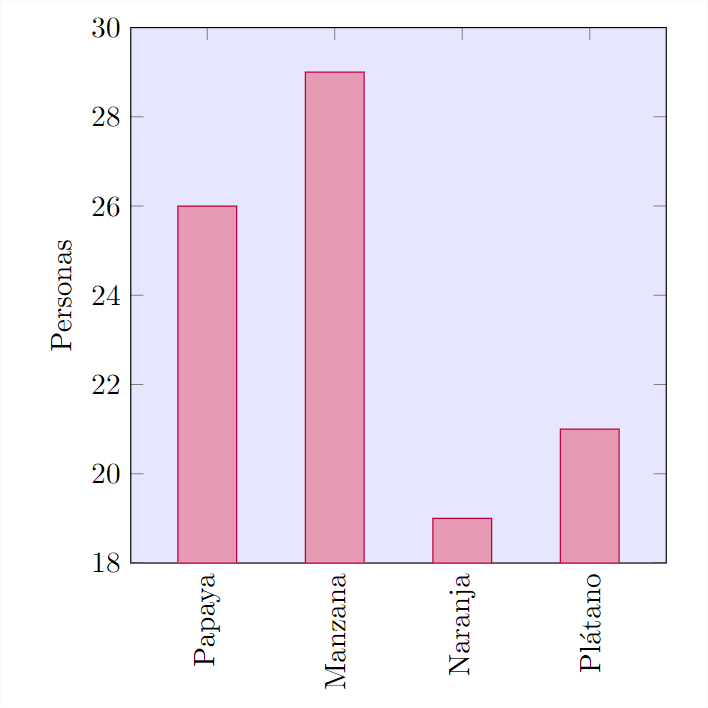
\includegraphics[width=.7\linewidth]{mexmat00001.png}
                              \end{parts}
                        \end{multicols}
                  }]

      \questionboxed[3]{Los resultados de una encuesta se muestran en la siguiente gráfica de barras:

            \begin{multicols}{2}
                  \begin{parts}
                        \part  ¿Cuántas personas participaron en la encuesta? \fillin[70][2cm]
                        \part  ¿Cuál es la fruta menos preferida por las personas? \fillin[Papaya][2cm]
                        \part  ¿Cuál es la fruta preferida por las personas? \fillin[Plátano][2cm]

                        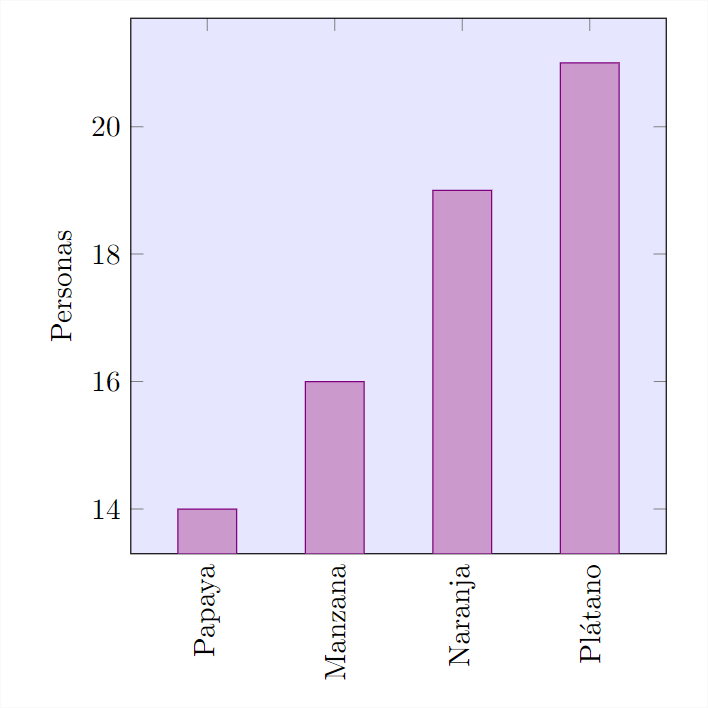
\includegraphics[width=.7\linewidth]{mexmat00001a.png}
                  \end{parts}
            \end{multicols}
      }

      % \newpage

      \section*{Círculo}
      \subsection*{Diámetro, Radio. Perímetro y Área de un círculo}

      \ejemplosboxed[{ Calcula el perímetro y área de los siguientes círculos:

                        \begin{multicols}{3}
                              \begin{parts}
                                    \part 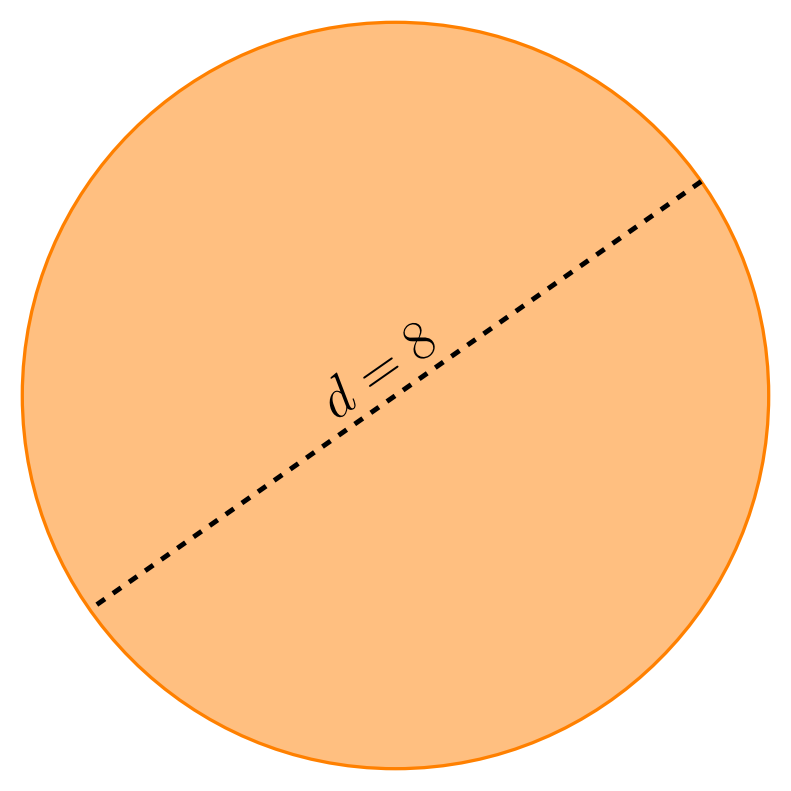
\includegraphics[width=0.9\linewidth]{mexmat00002.png}\\
                                    Perímetro: \fillin[25.12][0.3in] \ Área: \fillin[50.24][0.3in]

                                    \begin{solutionbox}{2cm}\footnotesize
                                          $P=8\pi=8(3.14)=25.12$ \\
                                          $A=\pi(4)^2=3.14(4)^2=50.24$
                                    \end{solutionbox}

                                    \part 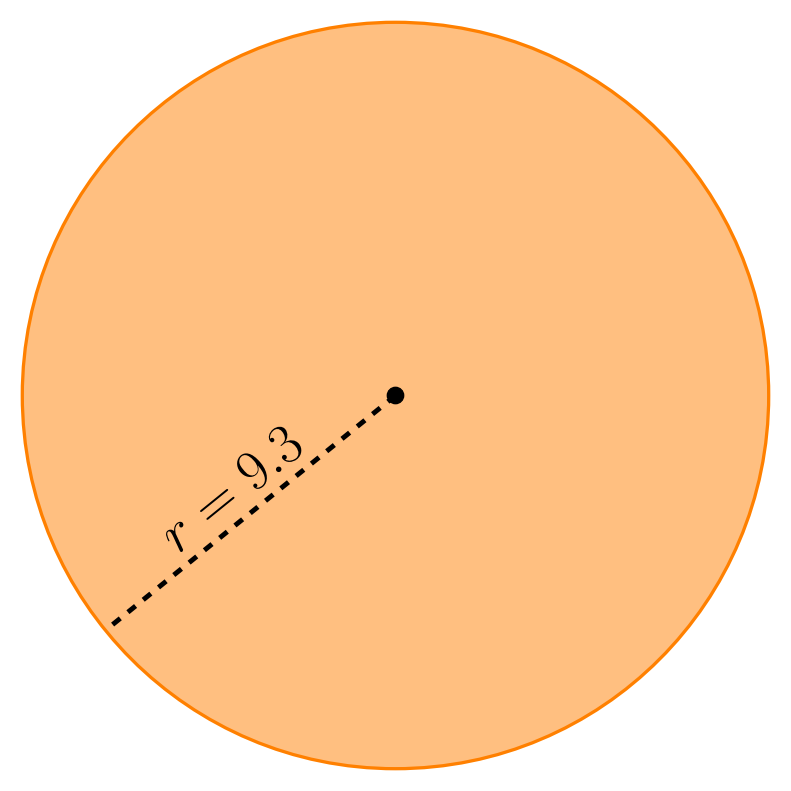
\includegraphics[width=0.9\linewidth]{mexmat00003.png}\\
                                    Perímetro: \fillin[58.40][0.3in] \ Área: \fillin[271.57][0.3in]

                                    \begin{solutionbox}{2cm}\footnotesize
                                          $P=2\pi r=2(3.14)(9.3)=58.4$ \\
                                          $A=\pi r^2=3.14(9.3)^2=271.57$
                                    \end{solutionbox}

                                    \part 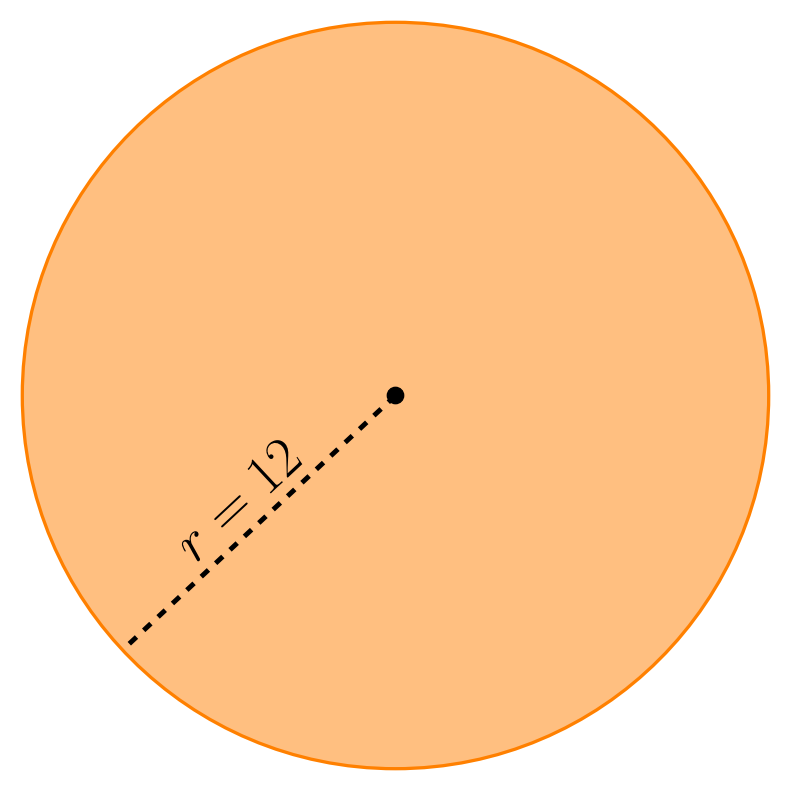
\includegraphics[width=0.9\linewidth]{mexmat00004.png}\\
                                    Perímetro: \fillin[75.36][0.3in] \ Área: \fillin[452.16][0.3in]

                                    \begin{solutionbox}{2cm}\footnotesize
                                          $P=2\pi r=2(3.14)(12)=75.36$ \\
                                          $A=\pi r^2=3.14(12)^2=452.16$
                                    \end{solutionbox}
                              \end{parts}
                        \end{multicols}

                  }]

      \questionboxed[9]{ Calcula el perímetro y área de los siguientes círculos:

            \begin{multicols}{3}
                  \begin{parts}
                        \part 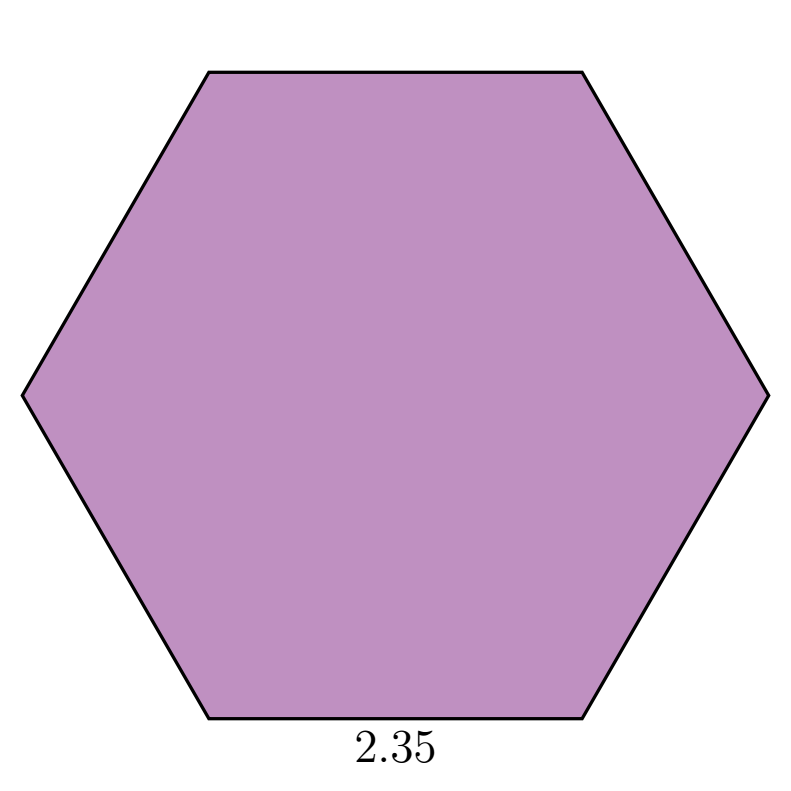
\includegraphics[width=0.85\linewidth]{mex_0007.png}\\
                        Perímetro: \fillin[][0.3in] \quad Área: \fillin[][0.3in]
                        \begin{solutionbox}{2cm}
                        \end{solutionbox}
                        \part 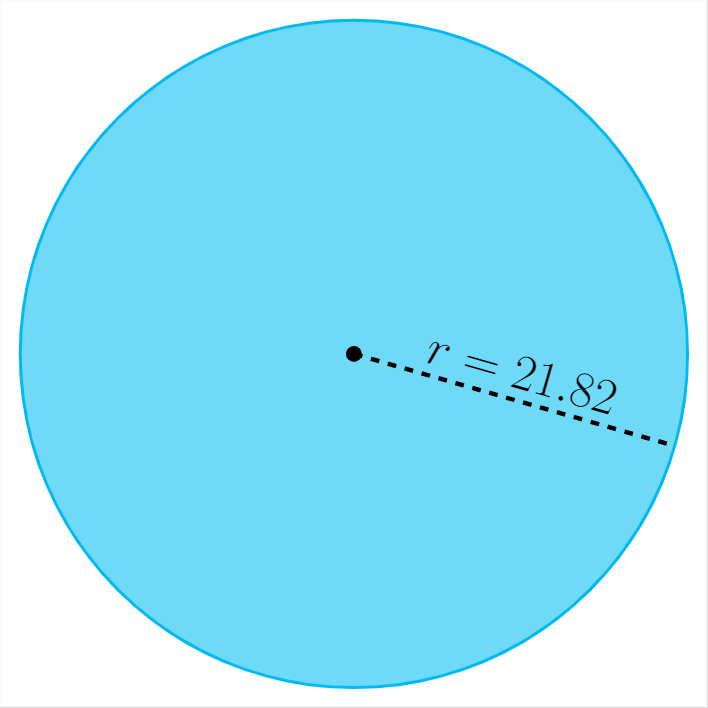
\includegraphics[width=0.85\linewidth]{mex_0008.png}\\
                        Perímetro: \fillin[][0.3in] \quad Área: \fillin[][0.3in]
                        \begin{solutionbox}{2cm}
                        \end{solutionbox}
                        \part 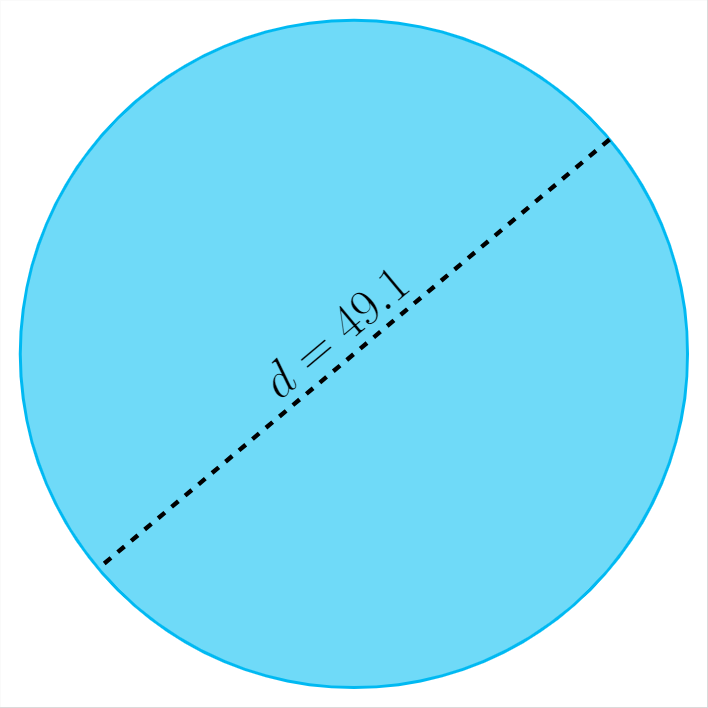
\includegraphics[width=0.85\linewidth]{mex_0009.png}\\
                        Perímetro: \fillin[][0.3in] \quad Área: \fillin[][0.3in]
                        \begin{solutionbox}{2cm}
                        \end{solutionbox}
                  \end{parts}
            \end{multicols}

      }

      \subsection*{Resolución de problemas}
      \ejemplosboxed[{Contesta las siguientes preguntas:

                        \begin{multicols}{2}
                              \begin{parts}
                                    \part Lisa tiene un terreno circular con un radio de 8 metros al cual le desea poner una barda en su periferia, si el precio por metro de barda es de 56 pesos. ¿Cuánto pagará en total por poner la barda?
                                    \$\fillin[2813.44][2cm]

                                    \begin{solutionbox}{2.2cm}
                                          $P=2\pi r=2(3.14)(8)=50.24$.\\
                                          Si cada metro cuesta \$56 \\
                                          $50.24\times56=2813.44$
                                    \end{solutionbox}

                                    \part Rodolfo quiere pintar una plataforma circular de 8 metros de radio, si el costo por pintar un metro cuadrado es de 98 pesos. ¿Cuánto pagará en total Rodolfo por pintar toda la plataforma?
                                    \$\fillin[19694.08][2cm]

                                    \begin{solutionbox}{2.2cm}
                                          $A=\pi r^2=3.14)(8)^2=200.96$. \\
                                          Si cada metro cuesta \$98 \\
                                          $200.96\times98=19694.08$
                                    \end{solutionbox}

                              \end{parts}
                        \end{multicols}
                  }]

      \questionboxed[4]{Contesta las siguientes preguntas:

            \begin{multicols}{2}
                  \begin{parts}

                        \part El radio de una rueda es de 32 centímetros, ¿cuántos centímetros habrá recorrido esa rueda después de haber dado 22 vueltas?
                        \fillin[$70737.92$ cm][0in]

                        \begin{solutionbox}{2cm}
                        \end{solutionbox}

                        \part Calcula el área de un parque que tiene un radio de 170 metros.
                        \fillin[$90746$ m][0in]

                        \begin{solutionbox}{2cm}
                        \end{solutionbox}

                  \end{parts}
            \end{multicols}
      }

      % \newpage

      \section*{Ecuaciones}
      \subsection*{Lenguaje algebraico}

      \ejemplosboxed[{Escribe la expresión algebraica correcta para los siguientes enunciados:

                        \begin{multicols}{2}
                              \begin{parts}
                                    \part El doble del cuadrado de un número.\\ \fillin[$2x^2$][0in]
                                    \part El cuadrado de la suma de dos números.\\  \fillin[$(x+y)^2$][0in]
                              \end{parts}
                        \end{multicols}
                  }]

      \questionboxed[4]{Escribe la expresión algebraica correcta para los siguientes enunciados:

            \begin{multicols}{2}
                  \begin{parts}
                        \part La mitad del cubo de un número.

                        \begin{solutionbox}{1.2cm}
                        \end{solutionbox}

                        \part Cinco veces un número menos cuatro unidades.

                        \begin{solutionbox}{1.2cm}
                        \end{solutionbox}
                  \end{parts}
            \end{multicols}
      }

      \subsection*{Ecuaciones x+a=b}
      \ejemplosboxed[{Resuelve las siguientes ecuaciones:

                        \begin{multicols}{3}
                              \begin{parts}
                                    \part $ x+7=12 $

                                    \begin{solutionbox}{2.8cm}
                                          \begin{align*}
                                                x+7 & = 12   \\
                                                x   & = 12-7 \\
                                                x   & = 5
                                          \end{align*}
                                    \end{solutionbox}

                                    \part $ x+182=-199 $

                                    \begin{solutionbox}{2.8cm}
                                          \begin{align*}
                                                x+182 & = -199     \\
                                                x     & = -199-182 \\
                                                x     & = -381
                                          \end{align*}
                                    \end{solutionbox}

                                    \part $ x-14=34 $

                                    \begin{solutionbox}{2.8cm}
                                          \begin{align*}
                                                x-14 & = 34    \\
                                                x    & = 34+14 \\
                                                x    & = 58
                                          \end{align*}
                                    \end{solutionbox}
                              \end{parts}
                        \end{multicols}
                  }]
      \questionboxed[6]{Resuelve las siguientes ecuaciones:

            \begin{multicols}{3}
                  \begin{parts}
                        \part $ x+7=-7 $

                        \begin{solutionbox}{1.8cm}
                        \end{solutionbox}

                        \part $ x-77=-192 $

                        \begin{solutionbox}{1.8cm}
                        \end{solutionbox}

                        \part $ x-50=-100 $

                        \begin{solutionbox}{1.8cm}
                        \end{solutionbox}
                  \end{parts}
            \end{multicols}
      }

      \subsection*{Ecuaciones ax=b}
      \ejemplosboxed[{Resuelve las siguientes ecuaciones:

                        \begin{multicols}{3}
                              \begin{parts}
                                    \part $ \dfrac{x}{10}=35 $

                                    \begin{solutionbox}{3cm}
                                          \begin{align*}
                                                \dfrac{x}{10} & = 35         \\
                                                x             & = 35\times10 \\
                                                x             & = 350
                                          \end{align*}
                                    \end{solutionbox}

                                    \part $ -2x=-24 $

                                    \begin{solutionbox}{3cm}
                                          \begin{align*}
                                                -2x & = 24             \\
                                                x   & = \dfrac{24}{-2} \\
                                                x   & = -12
                                          \end{align*}
                                    \end{solutionbox}

                                    \part $ 10x=-400 $

                                    \begin{solutionbox}{3cm}
                                          \begin{align*}
                                                10x & = -400            \\
                                                x   & =\dfrac{-400}{10} \\
                                                x   & = -40
                                          \end{align*}
                                    \end{solutionbox}
                              \end{parts}
                        \end{multicols}
                  }]
      \questionboxed[6]{Resuelve las siguientes ecuaciones:

            \begin{multicols}{3}
                  \begin{parts}
                        \part $ \dfrac{x}{-9}=9 $

                        \begin{solutionbox}{1.8cm}
                        \end{solutionbox}

                        \part $ -4x=20$

                        \begin{solutionbox}{1.8cm}
                        \end{solutionbox}

                        \part $ 8x=32 $

                        \begin{solutionbox}{1.8cm}
                        \end{solutionbox}
                  \end{parts}
            \end{multicols}
      }

      \subsection*{Ecuaciones ax+b=c}

      \ejemplosboxed[{Resuelve las siguientes ecuaciones:

                        \begin{multicols}{3}
                              \begin{parts}
                                    \part $ -x-2=15 $

                                    \begin{solutionbox}{3.8cm}
                                          \begin{align*}
                                                -x-2 & = 15                \\
                                                -x   & =15+2               \\
                                                -x   & =17                 \\
                                                x    & = \frac{17}{-1}=-17
                                          \end{align*}
                                    \end{solutionbox}

                                    \part $ 11x-33=55 $

                                    \begin{solutionbox}{3.8cm}
                                          \begin{align*}
                                                11x-33 & = 55            \\
                                                11x    & =55+33          \\
                                                11x    & =88             \\
                                                x      & = \frac{88}{11}
                                          \end{align*}
                                    \end{solutionbox}

                                    \part $ 4x-13=-25 $

                                    \begin{solutionbox}{3.8cm}
                                          \begin{align*}
                                                4x-13 & = -25              \\
                                                4x    & =-25+13            \\
                                                4x    & =-12               \\
                                                x     & = \frac{-12}{4}=-3
                                          \end{align*}
                                    \end{solutionbox}
                              \end{parts}
                        \end{multicols}
                  }]

      \questionboxed[6]{Resuelve las siguientes ecuaciones:

            \begin{multicols}{3}
                  \begin{parts}
                        \part $ -x-2=15 $

                        \begin{solutionbox}{3cm}
                        \end{solutionbox}

                        \part $ 11x-33=55 $

                        \begin{solutionbox}{3cm}
                        \end{solutionbox}

                        \part $ 4x-13=-25 $

                        \begin{solutionbox}{3cm}
                        \end{solutionbox}
                  \end{parts}
            \end{multicols}
      }

      % \subsection*{Resolución de problemas}



      \section*{Figuras y cuerpos geométricos}
      \subsection*{Perímetro y Área}

      \ejemplosboxed[{Encuentra el perímetro y el área de las siguientes figuras:

                        \begin{multicols}{3}
                              \begin{parts}
                                    \part Si la base del rectángulo mide 34.3 y su altura 28.
                                    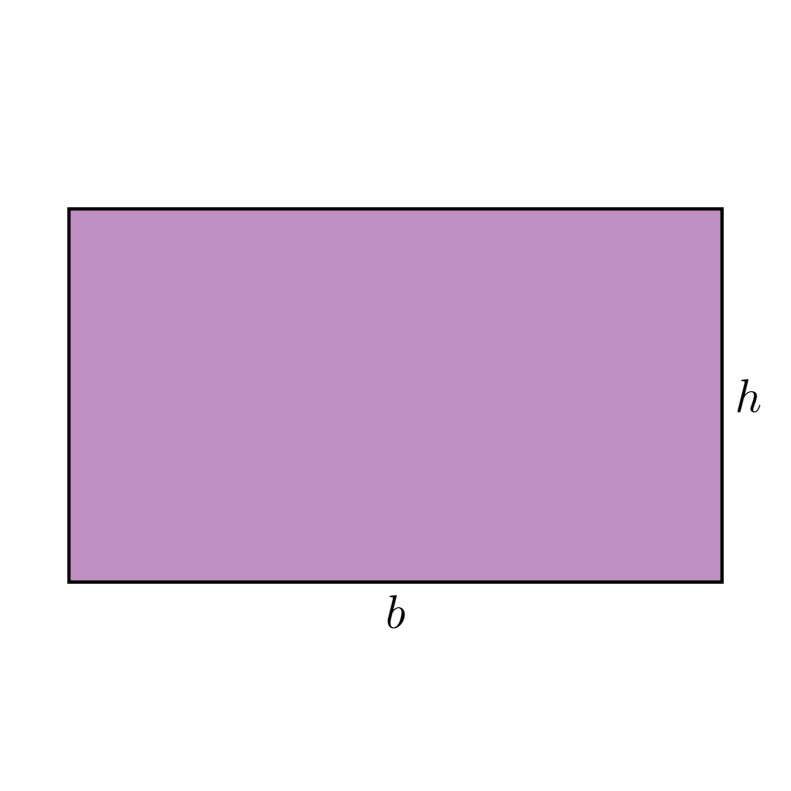
\includegraphics[width=0.9\linewidth]{mex_0019a.png}\\
                                    Perímetro: \fillin[124.6][0in] \  Área: \fillin[960.40][0in]

                                    % \begin{solutionbox}{1cm}
                                    % \end{solutionbox}

                                    \part Si el lado del polígono mide 32 y su apotema 12.
                                    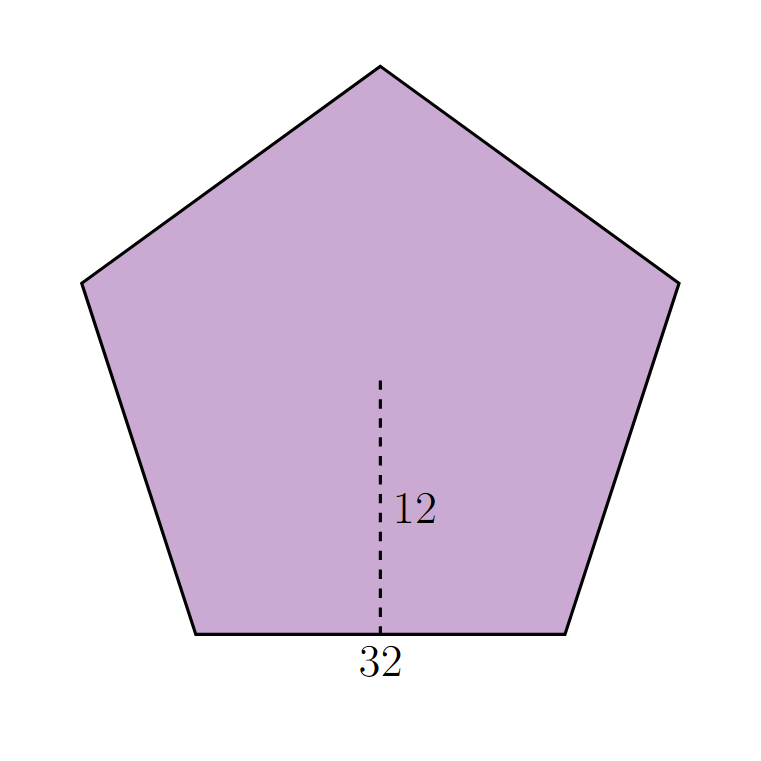
\includegraphics[width=0.8\linewidth]{mex_0018.png}\\
                                    Perímetro: \fillin[160][0in] \quad Área: \fillin[960][0in]

                                    % \begin{solutionbox}{1cm}
                                    % \end{solutionbox}

                                    \part Si el lado del polígono mide 9 y su apotema 18.
                                    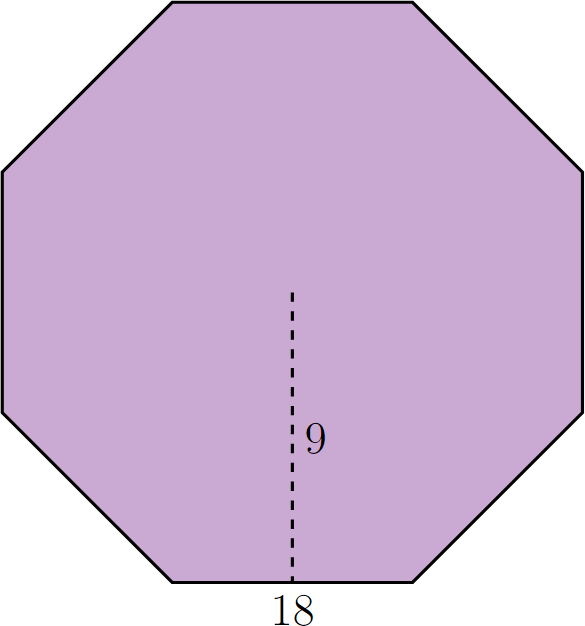
\includegraphics[width=0.9\linewidth]{mex_0016.png}\\
                                    Perímetro: \fillin[144][0in] \quad Área: \fillin[648][0in]

                                    % \begin{solutionbox}{1cm}
                                    % \end{solutionbox}
                              \end{parts}
                        \end{multicols}
                  }]

      \questionboxed[12]{Encuentra el perímetro y el área de las siguientes figuras:

            \begin{multicols}{3}
                  \begin{parts}
                        \part Si el lado del polígono mide 12 y su apotema 9.
                        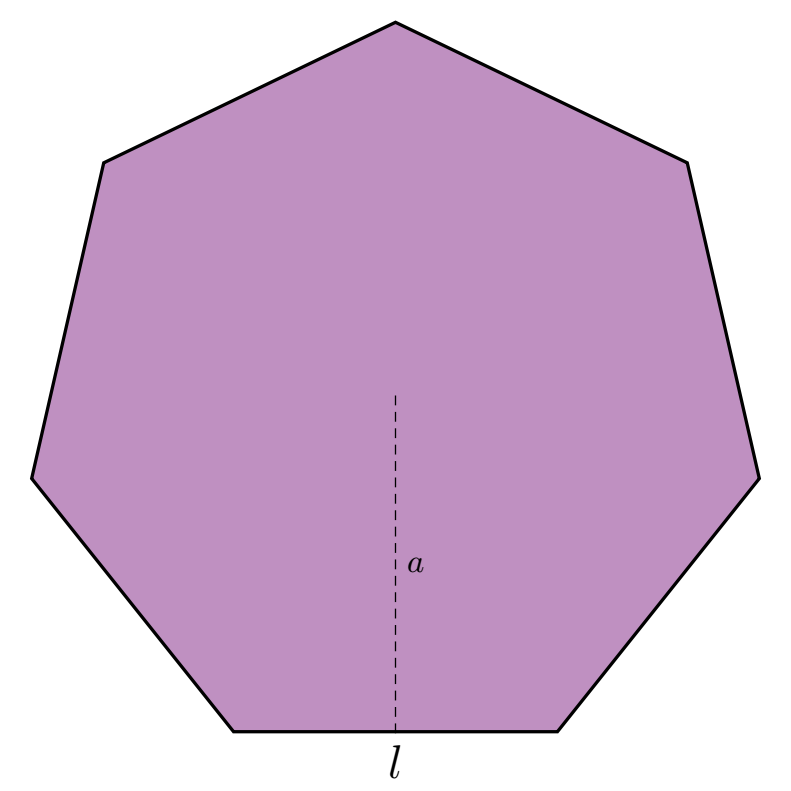
\includegraphics[width=0.8\linewidth]{mexmat00005.png}\\
                        Perímetro: \fillin[84][0.3in] \quad Área: \fillin[378][0.3in]

                        \begin{solutionbox}{1cm}
                        \end{solutionbox}

                        \part Si la base mayor del trapecio mide 33, su base menor 12 y su altura 14.
                        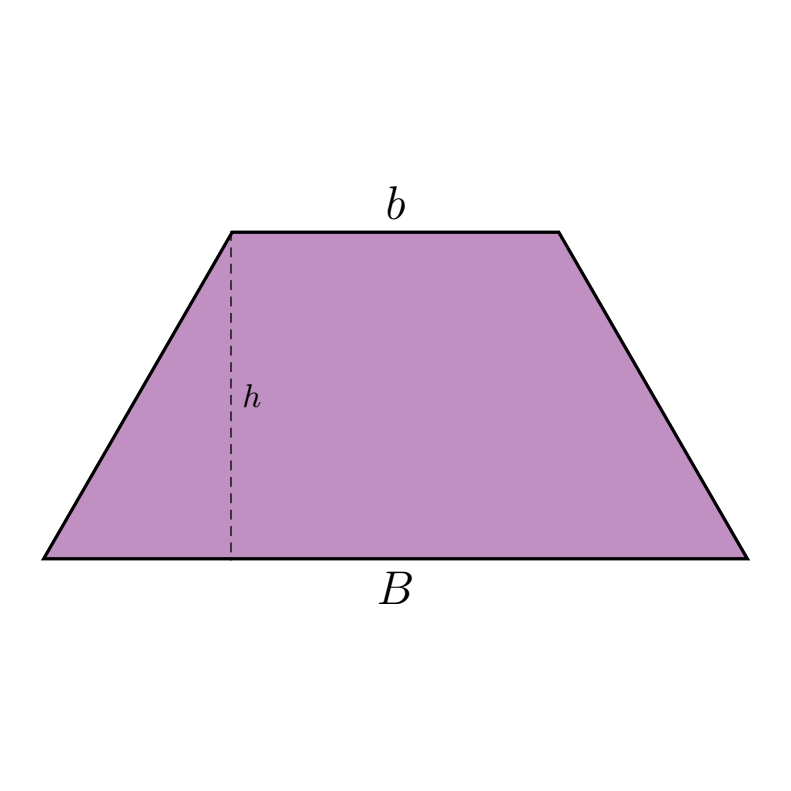
\includegraphics[width=0.9\linewidth]{mexmat00006.png}\\
                        Área: \fillin[][0.3in]

                        \begin{solutionbox}{1.5cm}
                        \end{solutionbox}

                        \part Si el lado del polígono mide 25 y su apotema 18.2.
                        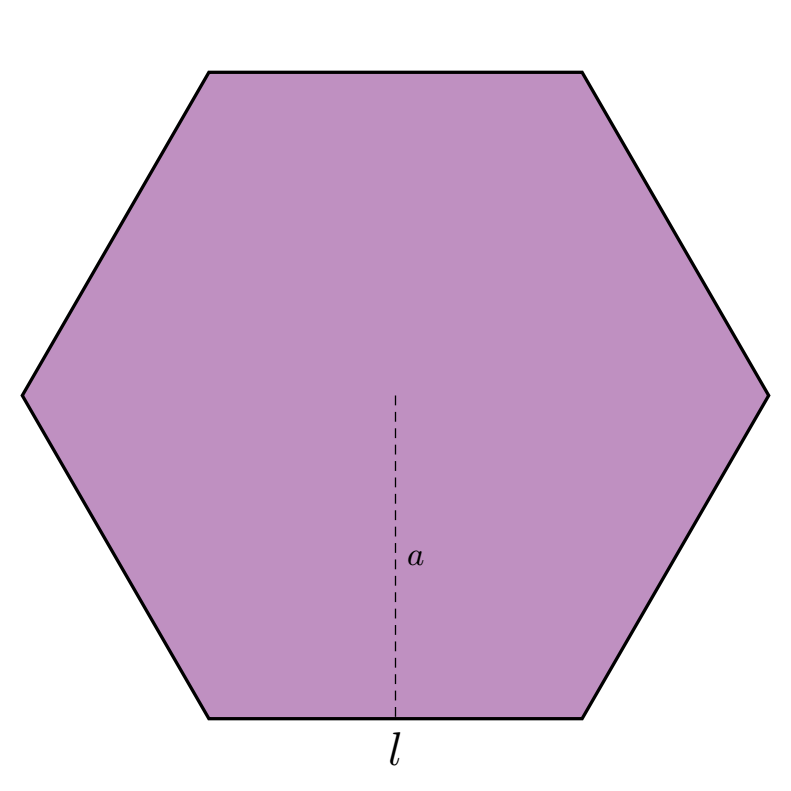
\includegraphics[width=0.8\linewidth]{mexmat00007.png}\\
                        Perímetro: \fillin[][0.3in] \quad Área: \fillin[][0.3in]

                        \begin{solutionbox}{1cm}
                        \end{solutionbox}


                  \end{parts}
            \end{multicols}
      }

      \subsection*{Área lateral,área total y volumen}

      \ejemplosboxed[{Calcula el volumen, el área lateral y el área total de las siguientes figuras:

                        \begin{multicols}{2}
                              \begin{parts}
                                    \part 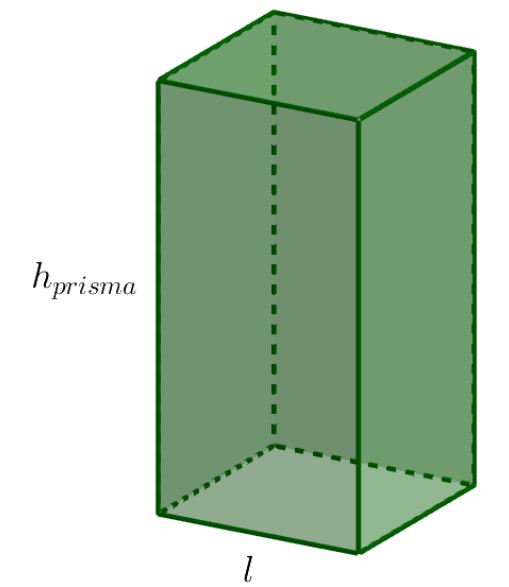
\includegraphics[width=0.65\linewidth]{mex_0026.png}\\
                                    Prisma cuyos lados "l" de la base miden 8 cm y la altura "h prisma" mide 21 cm.\\
                                    Volumen: \fillin[$1344$ cm$^3$][0.4in] \\A. Lateral: \fillin[$672$ cm$^2$][0.4in] \\ A. Total: \fillin[$800$ cm$^2$][0.4in]


                                    \part 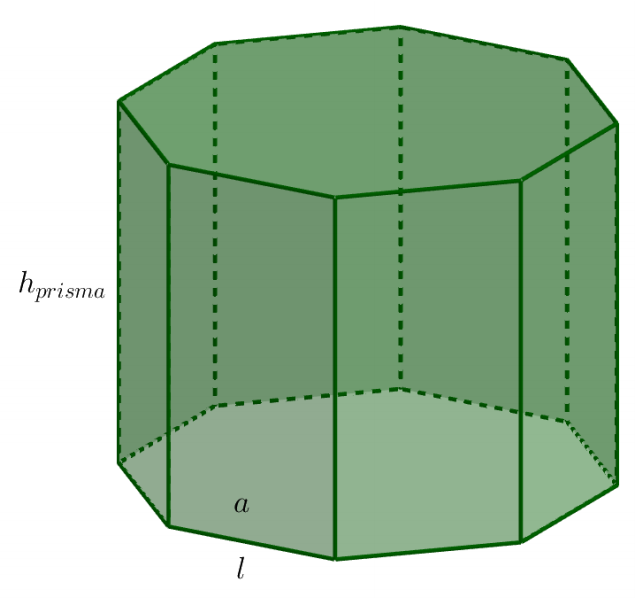
\includegraphics[width=0.65\linewidth]{mex_0025.png}\\
                                    Prisma de 19 cm de altura  y su base es un octágono cuyos los lados "l" miden 7 cm y tiene una apotema "a" de 5 cm.\\
                                    Volumen: \fillin[$2660$ cm$^3$][0.4in] \\A. Lateral: \fillin[$1064$ u][0.4in] \\ A. Total: \fillin[$1344$ cm$^2$][0.4in]
                              \end{parts}
                        \end{multicols}
                  }]

      \questionboxed[6]{Calcula el volumen, el área lateral y el área total de las siguientes figuras:

            \begin{multicols}{2}
                  \begin{parts}
                        \part 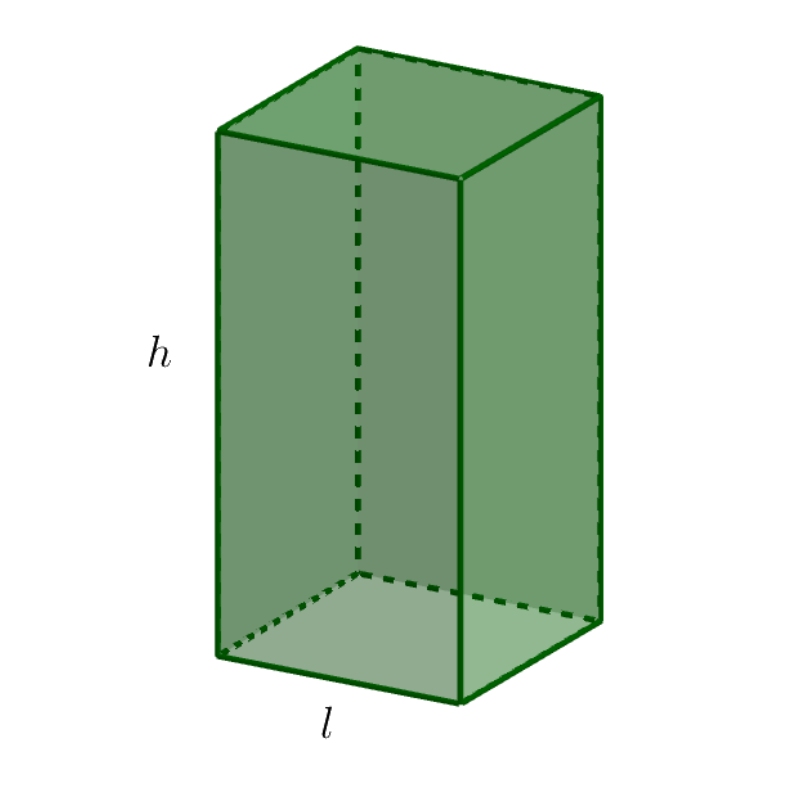
\includegraphics[width=0.65\linewidth]{mexmat00008.png}\\
                        Prisma cuyos lados "l" de la base miden 15 cm y la altura "h" mide 24 cm.

                        Área Lateral: \fillin[][0in]

                        \begin{solutionbox}{1cm}
                        \end{solutionbox}

                        Área Total: \fillin[][0in]

                        \begin{solutionbox}{1cm}
                        \end{solutionbox}

                        Volumen: \fillin[][0in]

                        \begin{solutionbox}{1cm}
                        \end{solutionbox}

                        \part 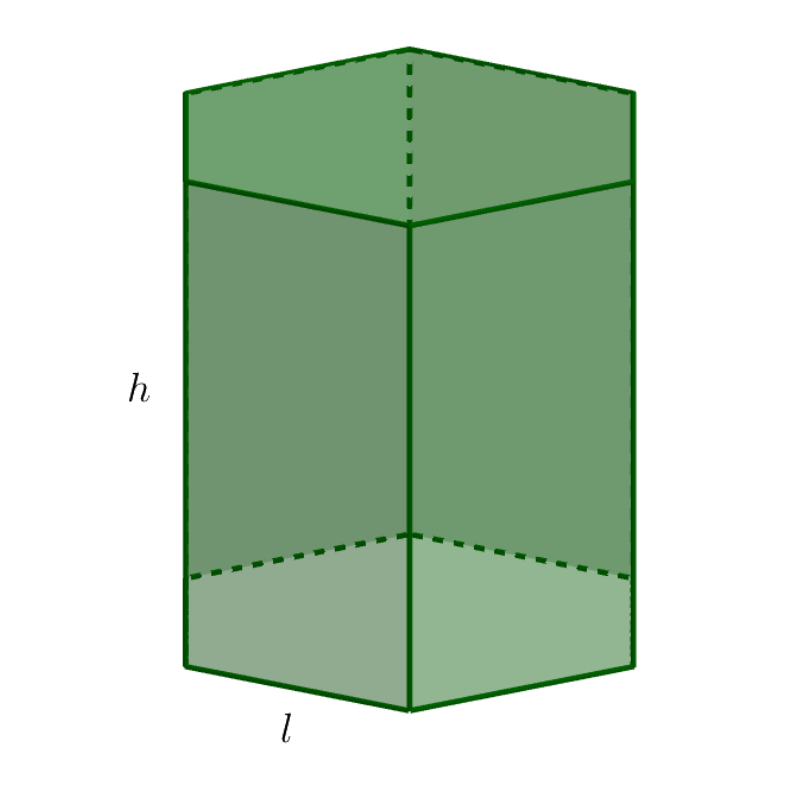
\includegraphics[width=0.65\linewidth]{mexmat00009.png}\\
                        Prisma cuyos lados "l" de la base miden 15.2 cm, el apotema mide 12.5 y la altura "h" mide 41.4 cm.

                        Área Lateral: \fillin[][0in]

                        \begin{solutionbox}{1cm}
                        \end{solutionbox}

                        Área Total: \fillin[][0in]

                        \begin{solutionbox}{1cm}
                        \end{solutionbox}

                        Volumen: \fillin[][0in]

                        \begin{solutionbox}{1cm}
                        \end{solutionbox}
                  \end{parts}
            \end{multicols}
      }

      % \subsection*{Resolución de problemas}

      % \questionboxed[6]{Resuelve los siguientes problemas:

      %     \begin{multicols}{3}
      %         \begin{parts}
      %             \part
      %             \begin{solutionbox}{2cm}
      %             \end{solutionbox}
      %             \part Ernesto compró 5 sandias, si pagó un total de 120 pesos por todas, ¿cuál es el costo de una sandia?
      %             \begin{solutionbox}{2cm}
      %             \end{solutionbox}
      %             \part Si al doble de un número le restamos 19 obtenemos 61, ¿qué número es?
      %             \begin{solutionbox}{2cm}
      %             \end{solutionbox}
      %         \end{parts}
      %     \end{multicols}
      % }

\end{questions}
\end{document}